\title{Solutions for Homework 4}
\author{Dr. Jordan Hanson - Whittier College Dept. of Physics and Astronomy}
\date{\today}
\documentclass[10pt]{article}
\usepackage[a4paper, total={18cm, 27cm}]{geometry}
\usepackage{graphicx}
\usepackage{amsmath}
\usepackage{tcolorbox}

\def\rcurs{{\mbox{$\resizebox{.16in}{.08in}{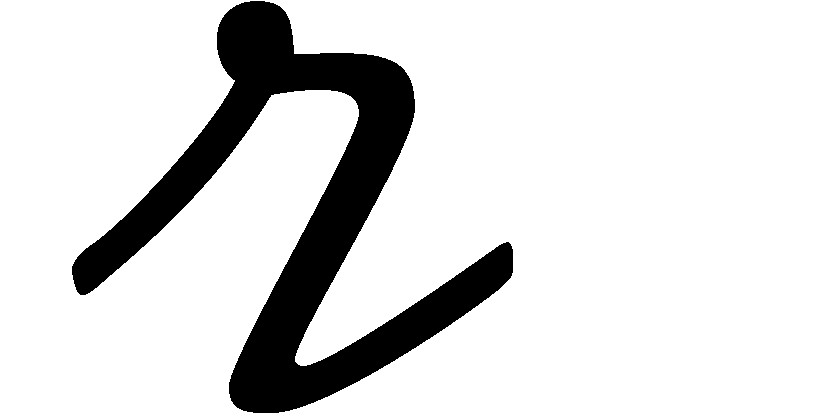
\includegraphics{ScriptR}}$}}}
\def\brcurs{{\mbox{$\resizebox{.16in}{.08in}{
\includegraphics{BoldR}}$}}}
\def\hrcurs{{\mbox{$\hat \rcurs$}}}

\begin{document}
\maketitle

\section{Problem 4.10}

\textit{A sphere of radius $R$ carries a polarization}
\begin{equation}
\mathbf{P}(\mathbf{r}) = k\mathbf{r} \label{eq:P}
\end{equation}
\textit{In Eq. \ref{eq:P}, $k$ is a constant and and $\mathbf{r}$ is the vector from the center.
\begin{itemize}
\item (a) Calculate the bound charges $\sigma_b$ and $\rho_b$.
\item (b) Find the field inside and outside the sphere.
\end{itemize}
}
(a) The surface bound charge is at radius $R$, so $\sigma_b = \mathbf{P} \cdot \hat{\mathbf{n}} = kR$.  The volumetric bound charge is $\rho_b = - \nabla \cdot \mathbf{P} = -3k$.  Note the total charge should add up to zero: $(4\pi R^2) \sigma_b + (4/3)\pi R^3 \rho_b = 4\pi R^3 k - 4\pi R^3 k = 0$. (b) The field of any constant volumetric charge density $-3k$ should be calculable via Gauss' law.  We find, after integrating over a Gaussian surface of radius $r<R$:
\begin{align}
\oint \mathbf{E} \cdot d\mathbf{a} = \mathbf{E} \cdot \mathbf{A} &= \frac{1}{\epsilon_0}\rho = \frac{-4k\pi r^3}{\epsilon_0} \\
\mathbf{E} &= -\frac{3kr}{\epsilon_0} \hat{\mathbf{r}} = -\mathbf{P}/\epsilon_0
\end{align}
(b) Note that, because the net charge is zero, the field outside the sphere is zero.

\section{Problem 4.14}

\textit{When you polarize a neutral dielectric, the charge moves a bit, but the total remains zero.  This fact should be reflected in the bound charges $\sigma_b$ and $\rho_b$.  Prove from Eqs. 4.11 and 4.12 that the toal bound charge vanishes.} \\

First, let's integrate the total volumetric bound charge:

\begin{equation}
-q = \int_{\mathcal{V}} \rho_b d\tau = -\int_{\mathcal{V}} \nabla \cdot \mathbf{P} d\tau = -\oint \mathbf{P} \cdot \hat{\mathbf{n}} da = -\oint \sigma_b da
\end{equation}

Next, the total surface bound charge is

\begin{equation}
q = \oint_S \sigma_b da
\end{equation}

Now we see that $Q = -q + q = 0$.

\section{Problem 4.15}

\textit{A thick spherical shell (inner radius a, outer radius b) is made of dielectric material with a frozen-in polarization}

\begin{equation}
\mathbf{P}(\mathbf{r}) = \frac{k}{r}\hat{\mathbf{r}} \label{eq:P2}
\end{equation}

In Eq. \ref{eq:P2}, $k$ is a constant and $r$ is the distance from the center.  There is no free charge in the problem.  Find the electric field in all three regions by two different methods:
\begin{itemize}
\item (a) Locate all the bound charge, and use Gauss' Law to calculate the field it produces.
\item (b) Use Eq. 4.23 to find $\mathbf{D}$, and then get $\mathbf{E}$ from Eq. 4.21. [Notice the second method is faster, and it avoids any explicit reference to the bound charges].
\end{itemize}

For (a), locating all the bound charge:

\begin{itemize}
\item $r = a$: 
\begin{equation}
\sigma_a = \mathbf{P} \cdot (- \hat{\mathbf{r}}) = -\left(\frac{k}{a}\right)\hat{\mathbf{r}}
\end{equation}
\item $a < r < b$:
\begin{equation}
\rho = -\nabla \cdot \mathbf{P} = -\frac{1}{r^2} \frac{\partial}{\partial r}\left(r^2 \frac{k}{r}\right) = -\frac{k}{r^2}
\end{equation}
\item $r = b$:
\begin{equation}
\sigma_b = \frac{k}{b}
\end{equation}
\item What is the total charge for this neutral object? 
\begin{equation}
Q = 4\pi(b - a) - 4\pi \int_a^b \rho d\tau = 4\pi(b-a) - 4\pi(b-a) = 0
\end{equation}
The neutral object has $Q = 0$.  Using Gauss' Law, $\mathbf{E} = 0$ for $r < a$, $\mathbf{E} = -\mathbf{P}/\epsilon_0$, and for $r > b$, $\mathbf{E} = 0$ because total charge is 0.
\end{itemize}

For (b), we find that since there is no free charge, $\mathbf{D} = 0$ and by the definition of $\mathbf{D}$, $\mathbf{E} = -\mathbf{P}/\epsilon_0$.  Thus, we achieve the same result by making reference to only the free charge.

\section{Problem 4.18}

\textit{The space between the plates of a parallel plate capacitor is filled with two slabs of linear dielectric material.  Each slab has thickness $a$, so the total distance between the plates is $2a$.  Slab 1 has a dielectric constant of $2$, and slab 2 has a dielectric constant of $1.5$.  The free charge density on the top plate is $\sigma$ and on the bottom plate $-\sigma$.}

\begin{itemize}
\item (a) Using Gauss' law for $\mathbf{D}$, we find that $\mathbf{D} = -\sigma \hat{\mathbf{z}}$ throughout the system.
\item (b) Using $\mathbf{D} = \epsilon \mathbf{E}$, we find slab 1 has $\mathbf{E} = - (\sigma/2\epsilon_0)\hat{\mathbf{z}}$ and slab 2 has $\mathbf{E} = -(2\sigma/3\epsilon_0) \hat{\mathbf{z}}$.
\item (c) Using the definition of $\mathbf{D}$, and the results from (b), we find $\mathbf{P} = - (\sigma/2)\hat{\mathbf{z}}$ for slab 1.  For slab 2 we find $\mathbf{P} = -(\sigma/3) \hat{\mathbf{z}}$.
\item (d) We know that $\Delta V = E \delta z = E_1 a + E_2 a = (E_1 + E_2)a = (7\sigma a)/(6\epsilon_0)$.
\item (e) There is no $\rho_b$ because the polarization densities are constant.  For the bound surface charges, there is $-\sigma/2$ at the top of slab 1, and $\sigma/2$ at the bottom of slab 1 from medium 1.  There is $-\sigma/3$ at the top of slab 2 from medium 2, and $\sigma/3$ at the bottom of slab 2 from medium 2.  At the interface, if we add surface charges, we find $\sigma/6$.
\item (f) To find the same fields as above, we must combine total charge from free and bound charges at the top and bottom surfaces.
\end{itemize}

\section{Problem 4.26}

\textit{A spherical conductor, of radius $a$, carries a charge $Q$.  It is surrounded by linear dielectric material of susceptibility $\chi_e$, out to radius $b$.  Find the energy of this configuration.}

The goal is to find $\mathbf{E}$ and $\mathbf{D}$, so that we can apply

\begin{equation}
W = \frac{1}{2}\int \mathbf{D} \cdot \mathbf{E} ~ d\tau \label{eq:W}
\end{equation}

The results are:

\begin{itemize}
\item Displacement inside the conductor ($r<a$): 0
\item Displacement outside the conductor ($r>a$): $Q/(4\pi r^2)\hat{\mathbf{r}}$
\item Field inside the conductor: 0
\item Field outside the conductor but inside the dielectric ($a<r<b$): $Q/(4\pi\epsilon r^2)\hat{\mathbf{r}}$.
\item Field outside the dielectric ($r>b$): $Q/(4\pi\epsilon_0 r^2)\hat{\mathbf{r}}$.
\end{itemize}

Inserting all these into into Eq. \ref{eq:W}, and integrating:

\begin{equation}
W = \frac{Q^2}{8\pi\epsilon_0(1+\chi_e)}\left( \frac{1}{a}+\frac{\chi_e}{b}\right)
\end{equation}

\section{Problem 4.35}

\textit{A point charge $q$ is in embedded at the center of a sphere of linear dielectric material (with susceptibility $\chi_e$ and radius $R$).  Find the electric field, the polarization, and the bound charge densities, $\sigma_b$ and $\rho_b$.  What is the total bound charge on the surface? Where is the compensating negative bound charge located?}

\begin{itemize}
\item Use Gauss' Law with electric displacement: $\mathbf{D} = q/(4\pi r^2)\hat{\mathbf{r}}$.
\item The electric field is then $\mathbf{E} = \mathbf{D}/\epsilon$, or
\begin{equation}
\mathbf{E} = \frac{q}{4\pi \epsilon_0 (1+\chi_e)r^2}\hat{\mathbf{r}}
\end{equation}
\item For polarization, note that linear dielectrics have $\mathbf{P} = \epsilon_0 \chi_e \mathbf{E}$, so
\begin{equation}
\mathbf{P} = \left(\frac{\chi_e}{1+\chi_e}\right)\mathbf{D}~=~\left(\frac{\chi_e}{1+\chi_e}\right)\left(\frac{q}{4\pi r^2}\right) \hat{\mathbf{r}}
\end{equation}
\item The surface and volume bound charge densities are:
\begin{align}
\sigma_b = \mathbf{P} \cdot \hat{\mathbf{r}} &= \left(\frac{\chi_e}{1+\chi_e}\right)D \\
\rho_b &= -\nabla \cdot \mathbf{P} = -q\left(\frac{\chi_e}{1+\chi_e}\right) \delta^3(\mathbf{r})
\end{align}
\item The total surface bound charge is $Q = q \left(\frac{\chi_e}{1+\chi_e}\right)$, but the negative compensating charge is at the origin:
\begin{equation}
Q = \int \rho_b d\tau = -q \left(\frac{\chi_e}{1+\chi_e}\right)
\end{equation}
\end{itemize}

\end{document}

